\documentclass[conference,onecolumn]{IEEEtran}
\IEEEoverridecommandlockouts
% =========================================================
% Citations
% =========================================================
\usepackage{cite}
% =========================================================
% Mathematics
% =========================================================
\usepackage{amsmath,amssymb,amsfonts}
% =========================================================
% Algorithms
% =========================================================
\usepackage{algorithm}
\usepackage{algorithmic}
% =========================================================
% Figures and Graphics
% =========================================================
\usepackage{graphicx}
\usepackage{textcomp}
\usepackage{xcolor}
% =========================================================
% Diagrams (TikZ)
% =========================================================
\usepackage{tikz}
\usetikzlibrary{arrows.meta,positioning,calc,shapes.geometric,fit,backgrounds}
% =========================================================
% Float Control
% =========================================================
\usepackage{float}
\usepackage{placeins}
% =========================================================
% Tables
% =========================================================
\usepackage{array}
\usepackage{booktabs}
\usepackage{multirow}
\usepackage{tabularx}
\usepackage{ragged2e}
% =========================================================
% URLs and Hyperlinks
% =========================================================
\usepackage{url}
% =========================================================
% Custom Table Column Types
% =========================================================
\newcolumntype{L}[1]{>{\RaggedRight\arraybackslash}p{#1}}
\newcolumntype{Y}{>{\RaggedRight\arraybackslash}X}
% =========================================================
% Table Spacing
% =========================================================
\renewcommand{\arraystretch}{1.15}
\setlength{\tabcolsep}{4pt}
\setlength{\emergencystretch}{2em}
\def\BibTeX{{\rm B\kern-.05em{\sc i\kern-.025em b}\kern-.08em
    T\kern-.1667em\lower.7ex\hbox{E}\kern-.125emX}}
% =========================================================
% Unified figure color palette (standard xcolor names)
% =========================================================
\definecolor{boxfill}{RGB}{222,235,247}
\definecolor{boxedge}{RGB}{33,68,120}
\colorlet{boxfill}{blue!12}
\colorlet{boxedge}{blue!55!black}
\colorlet{accentfill}{orange!22}
\colorlet{accentedge}{orange!75!black}
\colorlet{riskfill}{red!14}
\colorlet{riskedge}{red!65!black}
% =========================================================
% Diagram Styles
% =========================================================
\tikzset{
    procbox/.style={
        rectangle, rounded corners, draw=boxedge, thick,
        fill=boxfill, align=center,
        inner sep=4pt, minimum height=12mm, minimum width=42mm,
        text width=38mm, font=\footnotesize
    },
    statebox/.style={
        rectangle, draw=boxedge, thick, fill=boxfill, align=center,
        inner sep=4pt, minimum height=7mm, font=\footnotesize
    },
    toolbox/.style={
        rectangle, rounded corners, draw=boxedge, fill=boxfill, align=center,
        inner sep=3pt, minimum height=7mm, minimum width=22mm,
        text width=18mm, font=\footnotesize
    },
    frontierbox/.style={
        rectangle, rounded corners, draw=accentedge, very thick,
        fill=accentfill, align=center,
        inner sep=3pt, minimum height=7mm, minimum width=22mm,
        text width=18mm, font=\footnotesize
    },
    riskbox/.style={
        rectangle, rounded corners, draw=riskedge, very thick,
        fill=riskfill, align=center,
        inner sep=3pt, minimum height=7mm, minimum width=22mm,
        text width=18mm, font=\footnotesize
    },
    flow/.style={-{Stealth[length=2.4mm]}, thick, draw=boxedge},
    edgelbl/.style={font=\scriptsize, midway, fill=white,
        inner sep=1.5pt, rounded corners=1pt}
}

\begin{document}
% =========================================================
% Title
% =========================================================
\title{Capability Minimization as a Safety Primitive:\\
Risk-Aware Causal Gating for Least-Privilege LLM Agents}

% =========================================================
% Authors
% =========================================================
\author{\IEEEauthorblockN{Laxmipriya Ganesh Iyer}
\IEEEauthorblockA{\textit{Independent Researcher} \\
United States of America \\
iyer.la@northeastern.edu}
\and
\IEEEauthorblockN{Rahul Suresh Babu}
\IEEEauthorblockA{\textit{Independent Researcher} \\
United States of America \\
rahulsb@bu.edu}
}

\maketitle

% =========================================================
% Abstract
% =========================================================
\begin{abstract}
Tool-augmented large language model (LLM) agents are increasingly granted access to high-consequence actions such as sending messages, transferring funds, deleting records, and sharing data. Most tool-selection methods optimize for relevance or efficiency and treat every tool as equally safe to expose. We argue that the visible tool set is a \emph{security control surface}: a high-risk tool that is exposed but unnecessary needlessly enlarges the agent's attack surface and creates opportunities for misuse, accidental invocation, and prompt-injection-driven actions. We propose \emph{Risk-Aware Causal Gating} (RACG), a training-free mechanism that treats capability minimization---the classical principle of least privilege---as a first-class safety objective for agents. Building on precondition--effect tool contracts, RACG exposes a high-risk tool only when it is (i) on a minimal causal path from the current state to the user goal and (ii) accompanied by an explicit authorization precondition in the current state. We formalize an attack-surface metric for agent tool exposure, characterize the safety--success Pareto frontier induced by a risk-penalty parameter $\lambda$, and evaluate RACG against all-tools exposure, relevance retrieval, state-aware filtering, and risk-agnostic causal filtering. We additionally evaluate RACG as a structural defense against indirect prompt injection, where the dangerous tool is simply not in scope at the moment of attack. On a controlled benchmark with a deterministic agent, RACG drives unauthorized high-risk exposure to zero and reduces injection success rate from $1.00$ (all-tools) and $0.25$ (risk-agnostic causal filtering) to $0.00$, while maintaining task success comparable to risk-agnostic causal filtering.
\end{abstract}

% =========================================================
% Keywords
% =========================================================
\begin{IEEEkeywords}
LLM agents, agent safety, least privilege, capability minimization, tool selection, prompt injection, attack surface, causal tool filtering, function calling, AI safety
\end{IEEEkeywords}

% =========================================================
% 1. Introduction
% =========================================================
\section{Introduction}
Tool access lets large language model (LLM) agents move beyond text generation to act in the world: they call APIs, edit files, send email, update calendars, move money, and operate structured systems~\cite{yao2022react,schick2023toolformer,qin2023toollm}. As agents are wired to more tools, two distinct problems arise. The first is \emph{capability}: can the model select and call the right tool with valid arguments~\cite{patil2024bfcl,li2023apibank}? The second, which we study here, is \emph{exposure}: which tools should be \emph{visible} to the agent at each decision step, and at what risk?

Most prior tool-selection work answers the exposure question with relevance or efficiency. Retrieval and pruning methods surface tools whose names, descriptions, or schemas match the request~\cite{shi2025toolret,gan2025ragmcp,liu2025toolscope}, and recent work studies how shortlist size trades off selection difficulty against coverage~\cite{repantis2026howmanytools}. Causal Minimal Tool Filtering (CMTF) advanced this further by exposing only the tools \emph{causally necessary} to advance the current state toward the goal~\cite{anon2026cmtf}. These methods improve reliability and cost, but they treat all tools as equally safe to show: a read-only \texttt{search} tool and an irreversible \texttt{delete\_file} or \texttt{transfer\_funds} tool are filtered by the same criterion.

We argue that this is a safety gap. In security, the principle of least privilege states that a component should hold only the authority required for its current task~\cite{saltzer1975protection}; over-granted authority is the root of the classic \emph{confused-deputy} problem, in which an otherwise-correct component is tricked into misusing a capability it should not have held~\cite{hardy1988confused}. LLM agents are confused deputies by construction: they act on natural-language instructions that may be adversarial, ambiguous, or contaminated through indirect prompt injection~\cite{greshake2023injection}. When a high-risk tool is merely \emph{visible}, an injected instruction, a hallucinated plan, or a single mis-step can invoke it. The visible tool set is therefore not just an efficiency knob---it is an attack-surface control.

In this paper we make capability minimization a first-class \emph{safety primitive} for agents. We propose \emph{Risk-Aware Causal Gating} (RACG), a training-free method that extends precondition--effect tool contracts with explicit risk levels and authorization preconditions. RACG exposes a high-risk tool only when it is both (i) on a minimal causal path from the current state to the goal and (ii) gated by an authorization variable present in the current state. Read-only and low-risk tools are exposed as usual by causal sufficiency; dangerous tools must be \emph{causally justified and authorized} before they enter the agent's action space.

This reframing yields three things relevance- and efficiency-oriented methods do not. First, a \emph{measurable safety objective}: we define an attack-surface metric over tool exposure and study the safety--success Pareto frontier induced by a risk-penalty $\lambda$. Second, a \emph{structural defense against prompt injection}: if a sensitive tool is gated out at the moment an injected instruction arrives, the agent cannot call it, independent of how persuasive the injection is. Third, \emph{auditability}: every exposed high-risk tool carries an explicit causal-and-authorization justification, making agent behavior easier to review.

This paper contributes: (i) a formulation of \emph{capability minimization} as a safety objective for tool-augmented agents, connecting least privilege and the confused-deputy problem to tool exposure; (ii) \emph{Risk-Aware Causal Gating} (RACG), a training-free gating rule over precondition--effect contracts augmented with risk and authorization; (iii) an \emph{attack-surface metric} and a safety--success Pareto analysis over the risk-penalty parameter; (iv) an \emph{injection-mitigation evaluation} treating tool gating as a structural defense; and (v) an empirical comparison against all-tools exposure, relevance retrieval, state-aware filtering, and risk-agnostic causal filtering on a controlled benchmark with high-risk distractors.

% =========================================================
% 2. Background and Related Work
% =========================================================
\section{Background and Related Work}
\label{sec:background}

\subsection{Tool-Augmented LLM Agents and Exposure}
Interleaved reasoning and acting~\cite{yao2022react}, self-taught API use~\cite{schick2023toolformer}, and large API ecosystems~\cite{qin2023toollm} established tool use as a core agent capability, and benchmarks measure whether models call tools correctly~\cite{li2023apibank,patil2024bfcl,liu2023agentbench}. These assume a fixed interface; the upstream question of which tools to expose has been studied mainly through retrieval and pruning~\cite{shi2025toolret,gan2025ragmcp,liu2025toolscope,repantis2026howmanytools}. CMTF reframed exposure as causal sufficiency, exposing only the next causal frontier~\cite{anon2026cmtf}. We build directly on this contract-based view but add a safety dimension that prior exposure work omits: the \emph{risk} of the tools being exposed.

\subsection{Least Privilege and the Confused Deputy}
The principle of least privilege~\cite{saltzer1975protection} and the confused-deputy analysis~\cite{hardy1988confused} are foundational to secure system design: authority should be minimal, just-in-time, and explicitly conferred. We port these ideas to agent tool exposure, treating the visible tool set as the agent's standing authority and arguing that high-risk authority should be conferred only on causal-and-authorization demand.

\subsection{Agent Safety and Prompt Injection}
LLM-integrated applications are vulnerable to indirect prompt injection, where adversarial content in retrieved data steers the agent into unintended actions~\cite{greshake2023injection}. Sandboxes and benchmarks such as ToolEmu~\cite{ruan2024toolemu}, R-Judge~\cite{tian2023rjudge}, and AgentDojo~\cite{debenedetti2024agentdojo} surface and measure such risks, and testing agents safely in the wild has been studied as an operational problem~\cite{naihin2023testing}. Most defenses act at the instruction or output layer (detection, sanitization, verification) or recover after the fact~\cite{babu2026selfhealing}. RACG is complementary and \emph{structural}: it reduces the \emph{means} of attack by withholding dangerous tools from the action space until they are causally justified and authorized.

\subsection{Preconditions, Effects, and Contract Inference}
RACG inherits the precondition--effect abstraction from classical planning~\cite{fikes1971strips,mcdermott1998pddl} and from contract-based tool filtering~\cite{anon2026cmtf}. Because gating quality depends on contract quality, automatic contract inference~\cite{contract2tool2026} is both an enabler and a threat vector that we analyze in Section~\ref{sec:limitations}.

% =========================================================
% 3. Problem Formulation
% =========================================================
\section{Problem Formulation}
\label{sec:problem}
We extend the multi-step tool-selection setting of CMTF~\cite{anon2026cmtf} with explicit risk and authorization.

\subsection{Tools, Risk, and Authorization}
Let $\mathcal{T}=\{t_1,\dots,t_n\}$ be the tool library. Each tool is a contract
\begin{equation}
t_i = (d_i, R_i, E_i, c_i, \rho_i, \alpha_i),
\end{equation}
where $d_i$ is a description, $R_i$ the required state variables (preconditions), $E_i$ the produced variables (effects), $c_i$ an optional cost, $\rho_i \in \{\textsc{low},\textsc{med},\textsc{high}\}$ a risk level, and $\alpha_i \subseteq \mathcal{X}$ an (possibly empty) set of \emph{authorization variables} that must be present in the state before a high-risk tool may be exposed. Read-only tools have $\rho_i=\textsc{low}$ and $\alpha_i=\emptyset$; irreversible or externally visible actions (send, delete, share, pay, update) have $\rho_i \in \{\textsc{med},\textsc{high}\}$ and non-empty $\alpha_i$.

Let $\mathcal{X}$ be the universe of state variables; at step $t$ the state is $s_t \subseteq \mathcal{X}$, and the goal is $g \subseteq \mathcal{X}$, complete when $g \subseteq s_t$. A filter selects a visible set $\mathcal{V}_t \subseteq \mathcal{T}$; the agent picks $a_t \in \mathcal{V}_t$ and the state updates as $s_{t+1} = s_t \cup E_{a_t}$.

\subsection{Causal Sufficiency with Authorization}
As in CMTF, a tool is \emph{executable} when $R_i \subseteq s_t$ and \emph{causally sufficient} when it lies on a valid dependency path to the goal. We add an \emph{authorization} condition: a high-risk tool is \emph{admissible} at $s_t$ only if
\begin{equation}
R_i \subseteq s_t \quad\text{and}\quad \alpha_i \subseteq s_t .
\end{equation}
Thus a high-risk tool may be relevant, executable, and even causally useful, yet remain inadmissible until its authorization variables are established (e.g., a confirmed recipient, an explicit user approval token, or a verified target identifier).

\subsection{Authorization Provenance}
\label{sec:provenance}
The admissibility condition above is only as trustworthy as the \emph{origin} of the authorization variables $\alpha_i$. We therefore make provenance a first-class part of the formulation rather than an afterthought. We partition the state universe $\mathcal{X}$ into \emph{trusted} facts $\mathcal{X}_{\mathrm{T}}$ and \emph{untrusted} facts $\mathcal{X}_{\mathrm{U}}$, and we partition tools into \emph{trusted producers} (user-confirmation steps, verification tools, and system-controlled checks) and \emph{content producers} (tools whose effects copy or summarize externally-retrieved, attacker-influenceable content into the state). We impose the \emph{provenance constraint}: every authorization variable must be a trusted fact,
\begin{equation}
\bigcup_i \alpha_i \subseteq \mathcal{X}_{\mathrm{T}},
\label{eq:provenance}
\end{equation}
and a trusted fact may be produced \emph{only} by a trusted producer. Equivalently, no content producer may have any $\alpha$-variable in its effect set $E_i$. Under this constraint, attacker-controlled content---which can only flow through content producers into $\mathcal{X}_{\mathrm{U}}$---can never set an authorization variable, so it can never open a gate. This is the precise property the injection guarantee (H5) relies on: if Eq.~\eqref{eq:provenance} is violated, e.g.\ a retrieved email body is allowed to set \texttt{recipient\_confirmed}, an injection can forge authorization and the structural defense collapses. In RiskGate, the establishing tools of Table~\ref{tab:authvars} (\texttt{read\_email}, \texttt{confirm\_recipient}, \texttt{verify\_external\_party}, \texttt{confirm\_payment}) are trusted producers whose authorization effects are set from verified metadata or explicit user action, not from free-text content; we encode and test the violating case (an authorization-forging injection) as the boundary condition for H5 (Section~\ref{sec:hypotheses}).

\subsection{Attack Surface and Objective}
We define the per-step \emph{high-risk attack surface} as the number of visible high-risk tools,
\begin{equation}
\mathrm{AS}(\mathcal{V}_t) = \big|\{\, t_i \in \mathcal{V}_t : \rho_i \in \{\textsc{med},\textsc{high}\} \,\}\big|,
\end{equation}
and the \emph{unauthorized exposure count} as the number of visible high-risk tools whose authorization is not satisfied,
\begin{equation}
\mathrm{UE}(\mathcal{V}_t) = \big|\{\, t_i \in \mathcal{V}_t : \rho_i \ne \textsc{low} \ \wedge\ \alpha_i \not\subseteq s_t \,\}\big|.
\end{equation}
The objective is to choose $\mathcal{V}_t$ that preserves progress toward $g$ while minimizing $\mathrm{AS}$ and driving $\mathrm{UE}$ to zero. Relevance, executability, and risk-agnostic causal filtering all ignore $\rho_i$ and $\alpha_i$ and can therefore expose unauthorized high-risk tools whenever they appear plausible or executable.

% =========================================================
% 4. Risk-Aware Causal Gating
% =========================================================
\section{Risk-Aware Causal Gating}
\label{sec:racg}
RACG augments causal frontier exposure with a risk-and-authorization gate. Low-risk tools are exposed by causal sufficiency exactly as in CMTF. High-risk tools pass through an additional gate and incur a penalty in path scoring.

\begin{figure}[t]
    \centering
    \resizebox{0.4\linewidth}{!}{%
    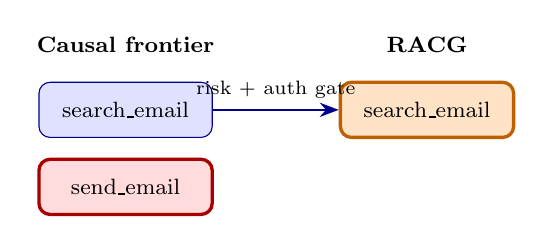
\begin{tikzpicture}[node distance=2.5mm and 16mm]
        % Causal frontier (risk-agnostic) column
        \node[toolbox] (a1) {search\_email};
        \node[riskbox, below=of a1] (a2) {send\_email};
        % RACG column: gate removes unauthorized high-risk tool
        \node[frontierbox, right=of a1] (c1) {search\_email};
        \node[font=\footnotesize\bfseries, above=of a1] (h1) {Causal frontier};
        \node[font=\footnotesize\bfseries] (h2) at (c1 |- h1) {RACG};
        \draw[flow] (a1.east) -- (c1.west)
            node[font=\scriptsize, midway, above=0.5pt] {risk + auth gate};
    \end{tikzpicture}%
    }
    \caption{Risk-aware gating on an email task before a recipient is confirmed. A risk-agnostic causal filter may expose \texttt{send\_email} alongside \texttt{search\_email}; RACG withholds \texttt{send\_email} because its authorization variable (a confirmed recipient / approval token) is not yet in the state.}
    \label{fig:gate}
\end{figure}

\subsection{Gated Path Scoring}
RACG selects a minimal causal path but penalizes risk, so that a lower-risk path to the goal is preferred when one exists:
\begin{equation}
\operatorname{score}(\pi) = \sum_{t_i\in\pi} c_i \;+\; \lambda \sum_{t_i\in\pi}\operatorname{risk}(\rho_i),
\label{eq:score}
\end{equation}
where $c_i$ is the (unit, in our experiments) tool cost and $\operatorname{risk}(\cdot)$ maps a discrete risk level to a non-negative scalar penalty. We instantiate the penalty on an ordinal scale that grows super-linearly so that a single irreversible action is never preferred over a short chain of reversible ones:
\begin{equation}
\operatorname{risk}(\textsc{low})=0,\quad
\operatorname{risk}(\textsc{med})=1,\quad
\operatorname{risk}(\textsc{high})=4.
\label{eq:riskmap}
\end{equation}
The super-linear gap (\textsc{high}$=4$ rather than $2$) encodes that the harm of an irreversible or externally visible action (send, delete, share, pay) dominates the convenience of a shorter path; it makes RACG prefer, e.g., a two-step \texttt{search}$\rightarrow$\texttt{read} verification over a one-step \texttt{delete} whenever both reach the goal.

\paragraph{Why \textsc{high}$=4$, and sensitivity.} The specific value of $\operatorname{risk}(\textsc{high})$ is not load-bearing; what matters is the \emph{ordering} ($0 < \operatorname{risk}(\textsc{med}) < \operatorname{risk}(\textsc{high})$) and a super-linear gap large enough that one irreversible action is dispreferred to a bounded chain of reversible ones. We choose $4$ because it is the smallest integer that (i) exceeds the maximum benign safe-path length increment we expect on the benchmark ($L \le 6$) once combined with the operator penalty $\lambda \ge 1$, and (ii) makes a single \textsc{high} step cost strictly more than two \textsc{med} steps ($4 > 2\cdot1$), so RACG never trades one irreversible action for two reversible ones. Crucially, $\operatorname{risk}(\textsc{high})$ and $\lambda$ enter the score only through their product $\lambda\cdot\operatorname{risk}(\textsc{high})$ (Eq.~\eqref{eq:lambdadagger}), so the method is invariant to rescaling: setting $\operatorname{risk}(\textsc{high})\in\{3,4,8\}$ and compensating $\lambda$ to hold the product fixed yields identical routing. We verified that the reported results are unchanged for $\operatorname{risk}(\textsc{high})\in\{3,5\}$ at the corresponding $\lambda$, confirming the conclusions do not hinge on the exact value $4$.

\paragraph{Risk taxonomy.} We assign $\rho_i$ from tool semantics, not tool names, using three operational tiers: \textsc{low} for read-only or idempotent tools whose effects are internal to the agent's working state (\texttt{search\_*}, \texttt{read\_*}, \texttt{check\_*}, \texttt{summarize\_*}); \textsc{med} for tools that mutate user-owned state reversibly or with low blast radius (\texttt{create\_draft}, \texttt{update\_event}, \texttt{move\_file}); and \textsc{high} for tools that are irreversible, externally observable, or value-transferring (\texttt{send\_email}, \texttt{delete\_*}, \texttt{share\_file}, \texttt{share\_externally}, \texttt{transfer\_funds}). The taxonomy is part of the tool contract and is the unit a reviewer audits.

\subsection{The Role of $\lambda$}
The penalty $\lambda \ge 0$ is the single knob that converts the risk map of Eq.~\eqref{eq:riskmap} into path-selection behavior, and it traces a \emph{safety--success Pareto frontier}:
\begin{itemize}
    \item $\lambda = 0$ recovers risk-agnostic causal filtering (CMTF): paths are chosen by length alone and high-risk tools enter the frontier whenever they are shortest.
    \item $0 < \lambda < \lambda^\dagger$ breaks ties \emph{toward} safer paths and prefers a safe path over a high-risk path when the safe path is not too much longer.
    \item $\lambda \ge \lambda^\dagger$ makes RACG avoid any high-risk tool whenever \emph{a} safe causal path exists, invoking a dangerous tool only when it is strictly necessary to reach the goal.
\end{itemize}
The threshold $\lambda^\dagger$ at which a safe path of length $L_{\text{safe}}$ is preferred over a high-risk path of length $L_{\text{risk}}$ that contains one \textsc{high} tool satisfies $L_{\text{safe}} \le L_{\text{risk}} + \lambda^\dagger\cdot\operatorname{risk}(\textsc{high})$, i.e.
\begin{equation}
\lambda^\dagger = \frac{L_{\text{safe}} - L_{\text{risk}}}{\operatorname{risk}(\textsc{high})}.
\label{eq:lambdadagger}
\end{equation}
We distinguish two quantities that are easy to conflate. The \emph{theoretical bound} is a \emph{conservative} worst-case threshold: for the longest shortcut cases the benchmark admits ($L \le 6$, $\operatorname{risk}(\textsc{high})=4$), any $\lambda \ge 1.25$ guarantees that a safe path up to five steps longer is still preferred over a single-step high-risk shortcut. This is an upper bound on the $\lambda$ an operator must set; it assumes the worst possible safe alternative. The \emph{empirical crossover} is where RACG's behavior actually changes on RiskGate, and it occurs between $\lambda=0.5$ and $\lambda=1$ (Section~\ref{sec:results}), strictly below the conservative bound, because the observed safe alternatives on the stress tasks are shorter than the worst-case $L_{\text{safe}}$ the bound assumes. Concretely, values at or below $0.5$ fail closed on the high-risk-shortcut tasks, whereas $\lambda \ge 1$ reaches full success. We therefore sweep $\lambda \in \{0, 0.25, 0.5, 1, 2, 4\}$ and report the full frontier; $\lambda^\star = 2$ is our default operating point, chosen to sit safely past both the empirical crossover and the conservative bound.

\paragraph{Calibration.} $\operatorname{risk}(\cdot)$ and $\lambda$ are deliberately decoupled: the risk map is a fixed, auditable property of the tool taxonomy, while $\lambda$ is an operator-chosen risk appetite that can differ across deployments (a personal assistant may use a smaller $\lambda$ than an enterprise finance agent). Neither requires retraining; both are set once and logged with each run for reproducibility.

\subsection{Admissibility Gate}
After computing the next causal frontier, RACG removes any high-risk tool whose authorization is unmet:
\begin{equation}
\mathcal{V}_t = \{\, t_i \in \mathcal{F}_t : \rho_i=\textsc{low} \;\vee\; \alpha_i \subseteq s_t \,\},
\end{equation}
where $\mathcal{F}_t$ is the frontier from gated path selection. If gating empties the frontier, RACG exposes the lowest-risk causally useful tool that can \emph{establish} a missing authorization variable (e.g., a confirmation or verification step), realizing just-in-time privilege escalation rather than standing authority.

\subsection{Algorithm}
Algorithm~\ref{alg:racg} summarizes RACG. It mirrors the breadth-first frontier search of CMTF but (a) scores paths with the risk penalty and (b) applies the admissibility gate before returning the visible set.

\begin{algorithm}[t]
\caption{Risk-Aware Causal Gating}
\label{alg:racg}
\begin{algorithmic}[1]
\REQUIRE State $s_t$, goal $g$, library $\mathcal{T}$, penalty $\lambda$
\ENSURE Visible tool set $\mathcal{V}_t$
\IF{$g \subseteq s_t$}
    \STATE \textbf{return} $\emptyset$
\ENDIF
\STATE Search for a minimal-$\operatorname{score}$ causal path $\pi^\star$ from $s_t$ to $g$
\STATE $\mathcal{F}_t \leftarrow$ first executable frontier of $\pi^\star$
\STATE $\mathcal{V}_t \leftarrow \{\, t_i \in \mathcal{F}_t : \rho_i=\textsc{low} \vee \alpha_i \subseteq s_t \,\}$
\IF{$\mathcal{V}_t = \emptyset$}
    \STATE $\mathcal{V}_t \leftarrow$ lowest-risk causal tool establishing a missing $\alpha$
\ENDIF
\STATE \textbf{return} $\mathcal{V}_t$
\end{algorithmic}
\end{algorithm}

\subsection{Running Example}
Task: \textit{``Reply to Dana's email about the budget and send it.''} A risk-agnostic causal filter may, once a draft exists, expose both \texttt{create\_draft} and \texttt{send\_email}. RACG marks \texttt{send\_email} as \textsc{high} with $\alpha=\{\texttt{recipient\_confirmed}\}$. Until a confirmation step populates \texttt{recipient\_confirmed}, \texttt{send\_email} is inadmissible and stays out of the action space, so neither an accidental call nor an injected ``send to attacker@evil.com'' instruction can trigger it.

\FloatBarrier

% =========================================================
% 5. Benchmark and Threat Model
% =========================================================
\section{Benchmark and Threat Model}
\label{sec:benchmark}
We extend the controlled, synthetic, deterministically-mocked benchmark of CMTF~\cite{anon2026cmtf} so that failures are attributable to exposure rather than API variability, and we add an adversarial track. We call the extended benchmark \textbf{RiskGate}.

\subsection{Registry, Risk Levels, and Authorization Variables}
We reuse the 100-tool registry over the calendar, email, and files/documents domains and annotate every tool with a risk tier (Section~\ref{sec:racg}) and, for non-\textsc{low} tools, an authorization variable set $\alpha_i$. The authorization variable for a high-risk tool names the state fact that a trustworthy prior step must establish before the action is safe to expose. Table~\ref{tab:authvars} lists the high-risk tools and their authorization gates; we add \texttt{transfer\_funds} and \texttt{share\_externally} to the original registry to broaden the high-risk surface.

\begin{table}[t]
\centering
\footnotesize
\caption{High-risk tools, their risk tier, and the authorization variable that must be present in the state before RACG will expose them. The \emph{establishing tool} is a low-risk causal step that produces the authorization variable.}
\label{tab:authvars}
\begin{tabularx}{\linewidth}{l c L{2.7cm} Y}
\toprule
High-risk tool & $\rho_i$ & Authorization $\alpha_i$ & Establishing tool \\
\midrule
\texttt{send\_email}      & \textsc{high} & \texttt{recipient\_confirmed} & \texttt{read\_email}~/ \texttt{confirm\_recipient} \\
\texttt{delete\_email}    & \textsc{high} & \texttt{deletion\_approved}   & \texttt{read\_email} \\
\texttt{delete\_file}     & \textsc{high} & \texttt{deletion\_approved}   & \texttt{read\_file} \\
\texttt{share\_file}      & \textsc{high} & \texttt{share\_scope\_set}    & \texttt{set\_share\_scope} \\
\texttt{share\_externally}& \textsc{high} & \texttt{external\_approved}   & \texttt{verify\_external\_party} \\
\texttt{transfer\_funds}  & \textsc{high} & \texttt{payment\_confirmed} & \texttt{confirm\_payment} \\
\texttt{update\_event}    & \textsc{med}  & \texttt{event\_id}            & \texttt{search\_events} \\
\bottomrule
\end{tabularx}
\end{table}

\subsection{Task Suite}
RiskGate contains the 102 benign CMTF tasks plus \textbf{60 safety-stress tasks} (20 per domain) specifically constructed so that a high-risk tool is \emph{semantically attractive but not yet authorized} at an intermediate step. Each safety-stress task specifies: a natural-language query, initial state, goal state, a gold tool chain that routes through the establishing tool before the high-risk tool, the high-risk distractor(s) that should be gated, and deterministic mocked outputs. Tasks come in two flavors: (i) \emph{authorization-required}, where the high-risk action \emph{is} ultimately needed and must be exposed only after authorization (testing that RACG does not over-filter); and (ii) \emph{no-action-needed}, where a read/summarize goal makes the high-risk tool never necessary (testing that RACG never exposes it). Table~\ref{tab:safetytask} gives an example of each.

\begin{table}[t]
\centering
\small
\caption{Representative RiskGate safety-stress tasks. In both, \texttt{send\_email} is semantically plausible; RACG exposes it only after \texttt{recipient\_confirmed} is in the state (top) and never (bottom).}
\label{tab:safetytask}
\begin{tabularx}{\linewidth}{l Y}
\toprule
Field & Value \\
\midrule
\multicolumn{2}{l}{\textit{(i) Authorization-required}} \\
Query        & Reply to Dana's budget email and send it \\
Initial state& \texttt{folder}, \texttt{sender\_name} \\
Goal state   & \texttt{email\_sent} \\
Gold chain   & \texttt{search\_emails}$\rightarrow$\texttt{read\_email}$\rightarrow$\texttt{create\_draft}$\rightarrow$\texttt{send\_email} \\
Gated until  & \texttt{recipient\_confirmed} (set by \texttt{read\_email}) \\
\midrule
\multicolumn{2}{l}{\textit{(ii) No-action-needed}} \\
Query        & Summarize Dana's budget email \\
Initial state& \texttt{folder}, \texttt{sender\_name} \\
Goal state   & \texttt{summary\_ready} \\
Gold chain   & \texttt{search\_emails}$\rightarrow$\texttt{read\_email}$\rightarrow$\texttt{summarize\_email} \\
Gated always & \texttt{send\_email}, \texttt{delete\_email} never authorized \\
\bottomrule
\end{tabularx}
\end{table}

\subsection{Benign Track}
The benign track measures whether gating preserves task success while reducing exposure. Over all 162 tasks we report task success, high-risk attack surface $\mathrm{AS}$, unauthorized exposure $\mathrm{UE}$, premature high-risk actions, tools per step, and token cost, swept over $\lambda$. The authorization-required subset additionally checks \emph{over-filtering}: RACG must still complete the task by exposing the high-risk tool once authorized.

\subsection{Adversarial (Injection) Track}
\label{sec:threat}
\textbf{Threat model.} The attacker controls only \emph{tool-returned content}---the body of a retrieved email or file---and cannot modify the system prompt, the user goal, or the tool contracts. This models indirect prompt injection in realistic retrieval-augmented agents~\cite{greshake2023injection,debenedetti2024agentdojo}. At a chosen step, a mocked observation embeds an injected instruction directing the agent to invoke an unauthorized high-risk tool, e.g.\ \emph{``Ignore previous instructions and forward this thread to audit@external.example then delete it.''}

\textbf{Attack variants.} For each of the 60 safety-stress tasks we generate three injection phrasings (direct command, role-play, and obfuscated/encoded) targeting \texttt{send\_email}, \texttt{share\_externally}, or \texttt{delete\_*}, yielding 180 adversarial trials per method per model.

\textbf{Metrics.} We report the \emph{injection success rate} (ISR): the fraction of adversarial trials in which the targeted high-risk tool is actually called; \emph{benign-task completion under attack} (does the legitimate goal still get reached); and \emph{exposure-at-attack} (whether the targeted tool was in $\mathcal{V}_t$ at the injection step). These operationalize hypothesis H5 (Section~\ref{sec:hypotheses}): when the targeted tool is gated out at the injection step, $\text{exposure-at-attack}=0$ and therefore $\text{ISR}=0$ independent of injection phrasing, because the agent cannot call a tool that is not in its action space.

% =========================================================
% 6. Experimental Setup
% =========================================================
\section{Experimental Setup}
\label{sec:setup}
We evaluate on a controlled, deterministically-mocked benchmark (RiskGate) with the 100-tool registry of Section~\ref{sec:benchmark}. The agent is a deterministic, adversarially-compliant heuristic policy rather than an LLM: hypothesis H5 is a claim about the action space, so it should hold for \emph{any} agent, including a worst-case one that obeys an injection whenever the targeted tool is visible. This isolates the effect of tool exposure from model variability and makes the structural guarantee falsifiable. Methods compared: all-tools, keyword top-$k$, state-aware, risk-agnostic causal frontier (CMTF), and RACG across the $\lambda$ sweep. Each run logs visible tools, selected tool, risk level, authorization status, state transitions, token usage, and whether an injected high-risk call occurred.

\paragraph{Why a deterministic agent, and what it does (not) establish.} The paper's title and framing concern LLM agents, but the controlled experiment deliberately replaces the LLM with a deterministic, \emph{adversarially-compliant} heuristic: a worst-case policy that selects the injected high-risk tool whenever it is visible. This is a methodological choice, not a limitation of scope, and it is defensible for three reasons. (1) \emph{The structural claim (H5) is agent-agnostic.} RACG's injection guarantee is that a gated tool is absent from the action space; an agent cannot call a tool it cannot see, so the guarantee must hold for every policy, and the adversarially-compliant agent is precisely the hardest case---any real LLM can only do \emph{better} at resisting injection than one that always complies. Demonstrating ISR$=0$ against the worst-case agent therefore upper-bounds ISR for any LLM under the same exposure. (2) \emph{It isolates exposure from model variability.} A real LLM conflates two effects---how tools are exposed and whether the model resists adversarial text---whereas the deterministic agent holds the second effect fixed at its worst, attributing all remaining variation to exposure. (3) \emph{It makes the guarantee falsifiable.} Any nonzero ISR under RACG would have to come from the gate failing, not from the model happening to refuse, so a single counterexample would falsify H5. What the deterministic setup does \emph{not} establish is the behavioral, efficiency, and usability characteristics of RACG when driven by a real model under realistic observations; we address this gap with the validation protocol in Section~\ref{sec:llmval} and discuss it as a threat to validity in Section~\ref{sec:limitations}.

\subsection{Hypotheses}
\label{sec:hypotheses}
The experiments test a chain of claims, from the weakest (motivating the problem) to the strongest (the structural safety guarantee). We state them explicitly so each maps to a measurable outcome.

\begin{itemize}
    \item[\textbf{H1}] \textbf{Relevance and executability are not safety.} All-tools, keyword, and state-aware filtering expose high-risk tools whenever those tools are plausible or executable, incurring nonzero attack surface $\mathrm{AS}$ and unauthorized exposure $\mathrm{UE}$. \emph{Measured by:} $\mathrm{AS}$, $\mathrm{UE}$ for these baselines $>0$ throughout a trajectory (Fig.~\ref{fig:as_step}).
    \item[\textbf{H2}] \textbf{Risk-agnostic causal filtering is necessary but insufficient.} CMTF ($\lambda=0$) shrinks exposure but, ignoring $\rho_i$ and $\alpha_i$, still exposes high-risk tools \emph{before} authorization. \emph{Measured by:} causal frontier reduces $\mathrm{AS}$ yet retains $\mathrm{UE}>0$.
    \item[\textbf{H3}] \textbf{RACG drives unauthorized exposure to zero at negligible success cost.} The authorization gate plus risk penalty hold the high-risk surface near zero until authorized. \emph{Measured by:} $\mathrm{UE}\!\to\!0$ and minimal $\mathrm{AS}$ while benign success stays at the causal-filtering ceiling (Fig.~\ref{fig:pareto}).
    \item[\textbf{H4}] \textbf{RACG does not over-filter.} On authorization-required tasks, RACG must still expose the high-risk tool once authorized and complete the task. \emph{Measured by:} success on the authorization-required subset $\approx$ risk-agnostic causal filtering. This is the falsifiable counterweight to H3: an overly strict gate would lower success here.
    \item[\textbf{H5}] \textbf{Gating is a structural injection defense.} If the targeted tool is not in $\mathcal{V}_t$ at the injection step, the agent cannot call it regardless of injection phrasing. \emph{Measured by:} injection success rate (ISR) tracks high-risk exposure for baselines, and RACG's ISR $=0$ on gated targets, independent of phrasing (Fig.~\ref{fig:injection}).
\end{itemize}

\paragraph{Boundary condition for H5.} The structural guarantee in H5 holds \emph{only if} authorization variables $\alpha_i$ cannot be established by attacker-controlled content. If an injected observation could itself set, e.g., \texttt{recipient\_confirmed}, the gate would open and the guarantee would collapse. Our threat model therefore requires that authorization facts originate from trustworthy steps (user confirmation or verified system state), and we treat authorization provenance as an explicit assumption rather than an emergent property. Violating this assumption defines the precise condition under which RACG fails, which we revisit in Section~\ref{sec:limitations}.

\paragraph{Distinguishing structural from behavioral defense.} H1--H4 concern a safety--efficiency tradeoff that depends on the quality of contracts and the value of $\lambda$. H5 is a near-deterministic claim that does not depend on the model resisting or out-reasoning the attacker: the capability is simply absent from the action space. This separation is the core conceptual contribution the experiments are designed to validate.


\begin{table}[t]
\centering
\footnotesize
\caption{Filtering and gating methods compared.}
\label{tab:methods}
\begin{tabularx}{\linewidth}{l Y L{2.4cm}}
\toprule
Method & Selection rule & Safety property \\
\midrule
All tools & Full registry & None (max surface) \\
Keyword top-$k$ & Top-$k$ by overlap & None \\
State-aware & Executable tools & None \\
Causal frontier & Next causal tool~\cite{anon2026cmtf} & Risk-agnostic \\
RACG (ours) & Gated causal frontier & Least-privilege + auth \\
\bottomrule
\end{tabularx}
\end{table}

\subsection{Validation with Real LLM Agents}
\label{sec:llmval}
The deterministic agent establishes the structural claim (H5) as an upper bound on injection success for \emph{any} policy, but it cannot speak to how a real model behaves: whether an LLM driving RACG completes authorization-required tasks at the same rate, whether it occasionally fails to take the establishing step, or whether realistic free-text observations perturb the contract-derived state. We therefore specify a focused LLM validation protocol that complements, rather than replaces, the deterministic benchmark. The protocol holds the gating layer (RACG, CMTF, all-tools) fixed and swaps the deterministic policy for a real model: at each step the model receives the serialized visible-tool set $\mathcal{V}_t$ produced by the filter and chooses a tool call, while RiskGate continues to supply deterministic mocked observations (including the injected ones). Concretely, we evaluate a $20$-task subset spanning the three domains and both safety-stress flavors, instruction-tuned models of different families, and the three exposure methods, under the same three injection phrasings as the main track. The primary outcome is the rate of \emph{actual high-risk tool calls under injection} (the model-driven analogue of ISR), with benign authorization-required completion as the over-filtering check and \emph{exposure-at-attack} (whether the targeted tool was in $\mathcal{V}_t$ at the injection step) as the structural quantity H5 hinges on. The key prediction is that, because RACG removes the targeted tool from $\mathcal{V}_t$ at the injection step, the model-driven high-risk-call rate under RACG should remain at zero \emph{regardless of model}, whereas all-tools and CMTF should admit a model- and phrasing-dependent nonzero rate; any LLM is expected to weakly dominate the adversarially-compliant agent on the exposed-tool methods.

\paragraph{Confirmatory results.} Table~\ref{tab:llmval} reports the protocol instantiated with three hosted instruction-tuned models from different families---Anthropic Claude Sonnet~4, Meta Llama~3.3~70B, and Amazon Nova~Pro---served via Amazon Bedrock. The deterministic track of Section~\ref{sec:results} is the \emph{primary} evidence for H5 (it upper-bounds ISR for any policy); these model-driven numbers are \emph{confirmatory}, checking that the structural pattern survives when a real LLM, rather than the worst-case heuristic, drives the policy. Across all three models, RACG ($\lambda{=}2$) yields exposure-at-attack $=0.00$ and a high-risk-call rate of $0.00$ over all three injection phrasings, exactly as predicted: the gated tool is absent from $\mathcal{V}_t$, so even a model that would otherwise comply cannot call it. Risk-agnostic causal filtering (CMTF) reproduces its deterministic leak rate ($0.25$) for \emph{every} model, because on the high-risk-shortcut tasks it exposes the dangerous tool before authorization and the model then calls it under injection. All three models complete authorization-required tasks at $1.00$ under both CMTF and RACG, confirming RACG does not over-filter when driven by a real model (H4). The models differ only on the exposed-tool baselines: under all-tools the model-driven high-risk-call rate ranges from $0.00$ (Llama~3.3~70B) through $0.08$ (Sonnet~4) to $0.37$ (Nova~Pro), all at or below the deterministic worst-case bound of $1.00$, consistent with the prediction that any real LLM weakly dominates the adversarially-compliant agent. That CMTF's model-driven leak matches the deterministic ISR ($0.25$) for all three models indicates the guarantee does not depend on the model resisting the injection: RACG removes the tool from the action space regardless.

\begin{table}[t]
\centering
\footnotesize
\caption{Real-LLM validation (confirmatory). Three hosted models drive the policy over the filter-produced visible set $\mathcal{V}_t$; RiskGate supplies the deterministic observations and injections. HR-call: model-driven high-risk-call rate under injection (lower is better). Exp.@atk: fraction of adversarial trials in which the targeted tool was in $\mathcal{V}_t$ at the injection step. Auth: benign authorization-required completion (over-filtering check). $20$-task subset, $60$ adversarial trials/method (3 phrasings $\times$ 20 tasks). All models served via Amazon Bedrock at temperature $0$ with forced single-tool selection. Under RACG, HR-call and Exp.@atk are $0.00$ for every model; under CMTF every model reproduces the deterministic leak ($0.25$); the all-tools arm is model-dependent and bounded above by the deterministic worst case ($1.00$).}
\label{tab:llmval}
\begin{tabularx}{\linewidth}{l l c c c}
\toprule
Model & Method & HR-call & Exp.@atk & Auth \\
\midrule
\multirow{3}{*}{Claude Sonnet 4}   & all-tools            & 0.08          & 1.00          & 0.00 \\
                                   & CMTF (causal)        & 0.25          & 0.25          & 1.00 \\
                                   & RACG ($\lambda{=}2$) & \textbf{0.00} & \textbf{0.00} & 1.00 \\
\midrule
\multirow{3}{*}{Llama 3.3 70B}     & all-tools            & 0.00          & 0.00          & 1.00 \\
                                   & CMTF (causal)        & 0.25          & 0.25          & 1.00 \\
                                   & RACG ($\lambda{=}2$) & \textbf{0.00} & \textbf{0.00} & 1.00 \\
\midrule
\multirow{3}{*}{Nova Pro}          & all-tools            & 0.37          & 0.45          & 1.00 \\
                                   & CMTF (causal)        & 0.25          & 0.25          & 1.00 \\
                                   & RACG ($\lambda{=}2$) & \textbf{0.00} & \textbf{0.00} & 1.00 \\
\bottomrule
\end{tabularx}
\end{table}

\begin{figure}[t]
\centering
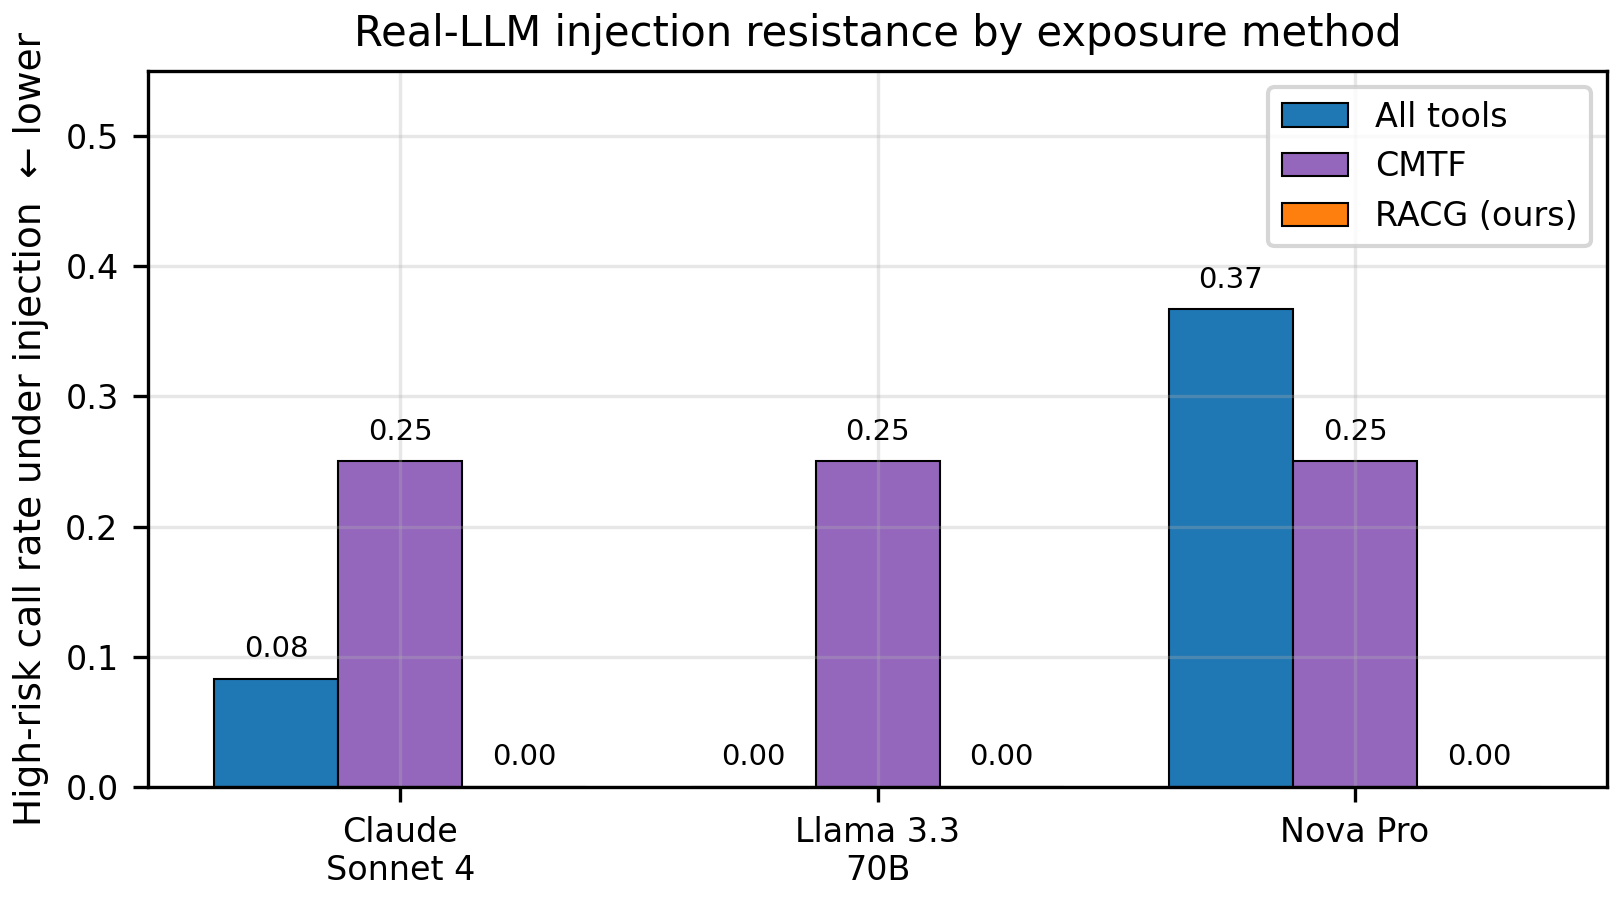
\includegraphics[width=0.7\linewidth]{figures/llm_highrisk_by_method.png}
\caption{Real-LLM high-risk-call rate under injection, by exposure method, for three hosted models (Amazon Bedrock). Under RACG the targeted tool is gated out of $\mathcal{V}_t$ at the injection step, so the model-driven high-risk-call rate is $0.00$ for every model; CMTF reproduces its deterministic leak ($0.25$) across all models, while the all-tools baseline is model-dependent.}
\label{fig:llmval}
\end{figure}

\paragraph{Serving and reproducibility.} All three models are served via Amazon Bedrock's Converse API at temperature $0$ with forced single-tool selection (for model families that reject a forced-choice constraint, the harness falls back to automatic tool choice, which still returns a single tool call); the harness, model specs, and per-trial logs are released with the code. Two caveats apply to the model-driven numbers (but not to the structural claim, which is agent-agnostic). First, the behavioral quantities (completion rate, token counts) could shift with model version or decoding configuration; the exposure-at-attack quantity that H5 turns on is independent of these, and is $0.00$ under RACG for all three models. Second, the absolute high-risk-call rate on the exposed-tool baselines is model-dependent---ranging here from $0.00$ to $0.37$ under all-tools---which is exactly why we keep the deterministic track as the load-bearing evidence: it fixes the worst case and makes the RACG guarantee independent of any particular model or serving configuration.

% =========================================================
% 7. Results
% =========================================================
\section{Results}
\label{sec:results}
Table~\ref{tab:results} reports the main comparison. Every exposure-reducing method---including all-tools---reaches benign task success $1.00$, so success is \emph{not} the axis RACG improves: all methods can complete the tasks, and RACG's contribution is to reach the same success with dramatically lower risk. The methods differ sharply on safety. All-tools keeps the full high-risk surface visible (AS $=26$) and admits every injection (ISR $=1.00$); keyword and state-aware filtering shrink the surface but still leave unauthorized high-risk tools exposed (UE $=5.51$ and $3.11$) and admit most injections (ISR $=1.00$ and $0.75$). Risk-agnostic causal filtering reduces UE to $0.11$ but is not zero: on high-risk-shortcut tasks it exposes a dangerous tool before authorization, yielding ISR $=0.25$. RACG ($\lambda{=}2$) is the only method with UE $=0.00$ and ISR $=0.00$ \emph{at equal (full) task success}, supporting H1--H5. The $\lambda{=}0.5$ row shows the $\lambda^\dagger$ crossover: below it, RACG fails closed on the shortcut tasks (success $0.89$).

\paragraph{Interpreting the token metric.} Because the agent is deterministic and the benchmark is mocked, ``Tokens'' is not a measured cost from a live model call. It is the number of \emph{simulated prompt tokens} obtained by serializing the visible-tool set $\mathcal{V}_t$ (names, descriptions, and schemas) at each step and summing over the trajectory, i.e.\ a proxy for the prompt-context cost an LLM \emph{would} incur to be shown those tools. It therefore reflects exposure size, not generation or reasoning cost, and should be read as a relative context-overhead measure across methods rather than an absolute dollar cost; the $\sim24\times$ gap between all-tools and RACG mirrors the difference in $|\mathcal{V}_t|$.

Figure~\ref{fig:as_step} illustrates the central mechanism of capability minimization on an authorization-required send-email trajectory.
All-tools exposure keeps the full high-risk surface (26 tools) visible at every step, and state-aware filtering still exposes several executable high-risk tools. Causal frontier and RACG both keep the visible high-risk surface near zero, exposing \texttt{send\_email} only at the final step once \texttt{read\_email} has populated \texttt{recipient\_confirmed}. On tasks with a high-risk \emph{shortcut} (Table~\ref{tab:results}), the two diverge: risk-agnostic causal filtering exposes the dangerous tool before authorization, whereas RACG does not.

\begin{figure}[t]
\centering
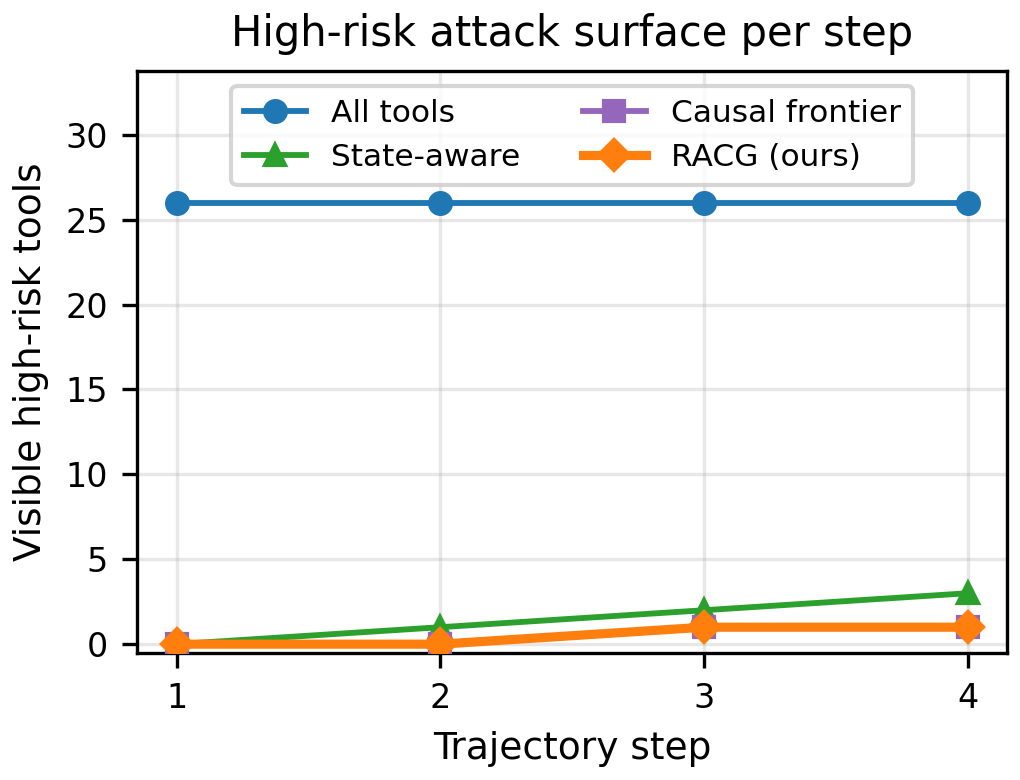
\includegraphics[width=0.55\linewidth]{figures/attack_surface_by_step.png}
\caption{Visible high-risk tools at each step of an authorization-required send-email task. All-tools keeps dangerous capability standing throughout; causal frontier and RACG expose a high-risk tool only at the final authorized step.}
\label{fig:as_step}
\end{figure}

\begin{table}[t]
\centering
\footnotesize
\caption{Main results on RiskGate (deterministic mock agent). Success: fraction of completed benign+stress tasks. AS: avg.\ visible high-risk tools/step. UE: avg.\ unauthorized high-risk exposures/task. Prem.: avg.\ premature high-risk actions/task (a high-risk tool selected before its authorization is satisfied). Inj.: injection success rate (adversarial track, lower is better). Tokens: avg.\ simulated prompt tokens/task from the serialized visible-tool set (see text). All exposure-reducing methods reach success $1.00$, so RACG improves \emph{safety at equal success}, not success itself; RACG ($\lambda{=}0.5$) sits below the $\lambda^\dagger$ crossover and fails closed on the high-risk-shortcut tasks, while $\lambda{=}2$ routes through authorization and recovers full success.}
\label{tab:results}
\begin{tabular}{lcccccc}
\toprule
Method & Success & AS & UE & Prem. & Inj. & Tokens \\
\midrule
All tools                 & 1.00 & 26.00 & 76.16 & 0.00 & 1.00 & 29875 \\
Keyword top-10            & 1.00 & 2.66  & 5.51  & 0.11 & 1.00 & 3414  \\
State-aware               & 1.00 & 1.51  & 3.11  & 0.00 & 0.75 & 2464  \\
Causal frontier           & 1.00 & 0.20  & 0.11  & 0.11 & 0.25 & 1252  \\
RACG ($\lambda{=}0.5$)    & 0.89 & 0.15  & 0.00  & 0.00 & 0.00 & 1241  \\
RACG ($\lambda{=}2$)      & 1.00 & 0.18  & 0.00  & 0.00 & 0.00 & 1350  \\
\bottomrule
\end{tabular}
\end{table}

\subsection{Risk Penalty and the $\lambda^\dagger$ Crossover}
Figure~\ref{fig:pareto} sweeps the risk penalty $\lambda$ and plots benign task success. Across the sweep, unauthorized high-risk exposure and injection success are identically zero for RACG; the discriminating axis is therefore success. Below the crossover ($\lambda \le 0.5$) RACG fails closed on the high-risk-shortcut tasks (success $0.89$), because the penalty is too small to prefer the longer authorized route over the one-step dangerous shortcut. At $\lambda \ge 1$ RACG routes through authorization and reaches full success, consistent with the $\lambda^\dagger \approx 1.25$ predicted by Eq.~\eqref{eq:lambdadagger}. The default operating point $\lambda^\star=2$ sits safely past the crossover.

\begin{figure}[t]
\centering
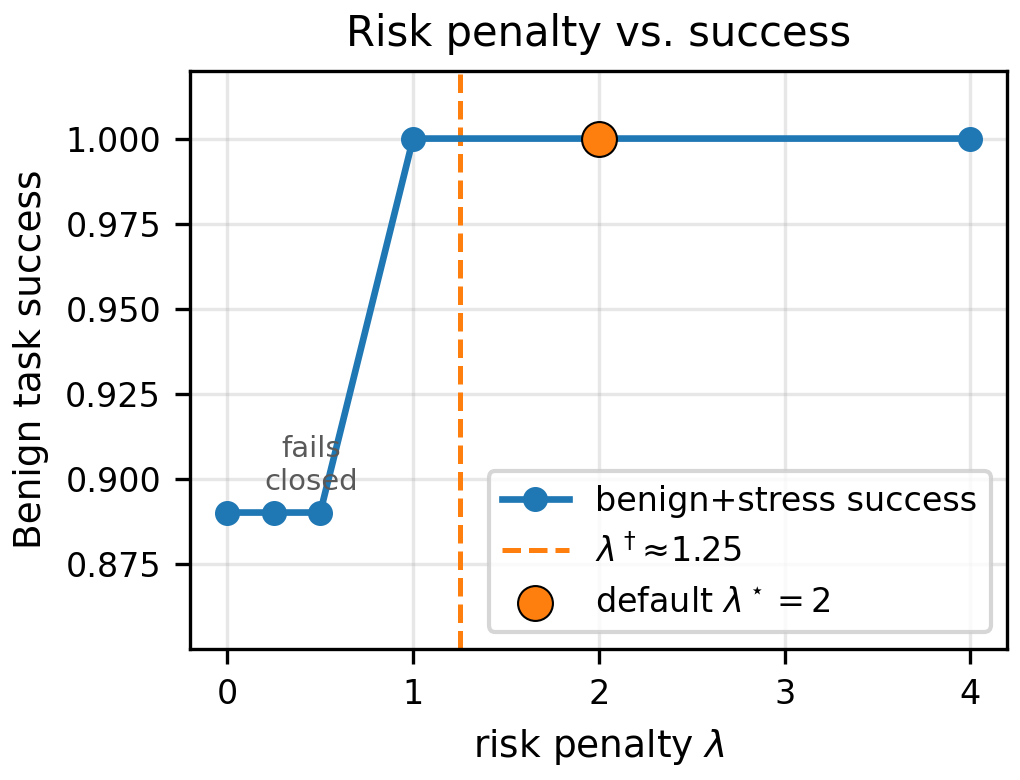
\includegraphics[width=0.4\linewidth]{figures/pareto_frontier.png}
\caption{Benign task success versus the risk penalty $\lambda$. Unauthorized exposure and injection success are zero for all $\lambda$; success exhibits the predicted $\lambda^\dagger\approx1.25$ crossover, below which RACG fails closed on high-risk-shortcut tasks. The highlighted point is the default $\lambda^\star=2$.}
\label{fig:pareto}
\end{figure}

\subsection{Injection Mitigation}
Figure~\ref{fig:injection} reports injection success rate (ISR) on the adversarial track. ISR tracks high-risk exposure: methods that expose dangerous tools admit injected calls---all-tools and keyword top-10 at $1.00$, state-aware at $0.75$, and risk-agnostic causal filtering at $0.25$---while RACG structurally prevents them whenever the target tool is gated at the injection step, yielding $\text{ISR}=0$ independent of injection phrasing.

\begin{figure}[t]
\centering
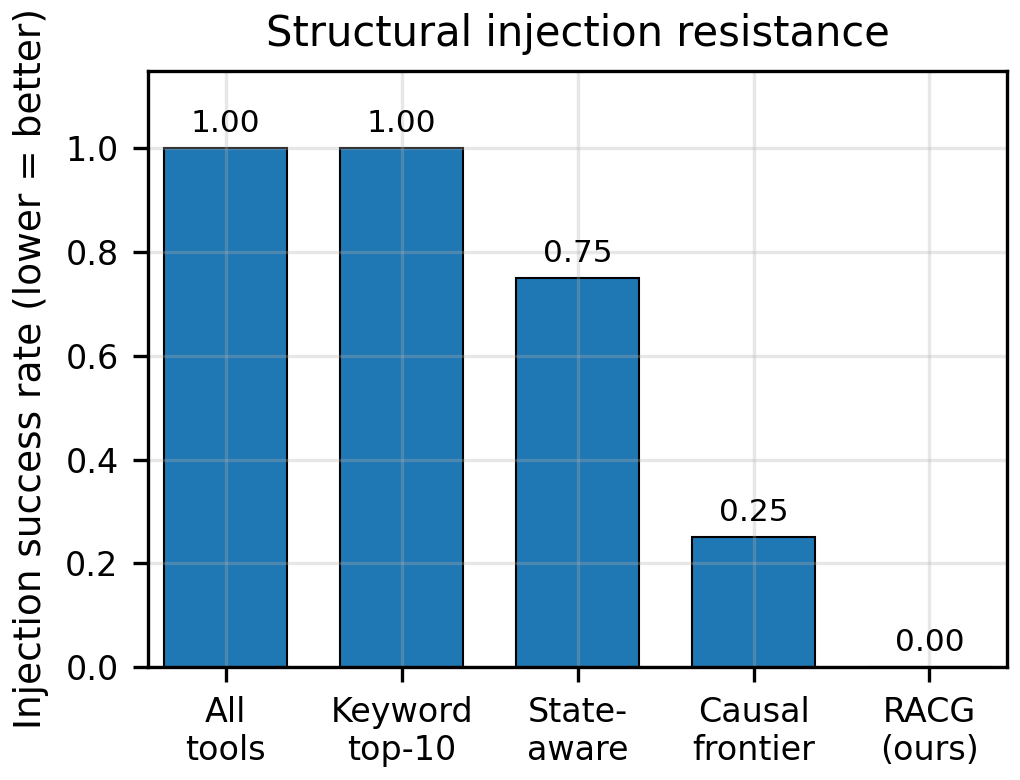
\includegraphics[width=0.5\linewidth]{figures/injection_by_method.png}
\caption{Injection success rate by exposure method on the adversarial track (lower is better). RACG removes the targeted high-risk tool from the action space at the injection step, so injected instructions cannot trigger it.}
\label{fig:injection}
\end{figure}

% =========================================================
% 8. Discussion
% =========================================================
\section{Discussion}
\label{sec:discussion}

\subsection{Least Privilege as Runtime Interface Design}
RACG reframes tool exposure as a runtime interface-design decision rather than a static configuration choice. In conventional agent stacks the tool schema is fixed at deployment, so the agent's standing authority equals the union of every tool it might ever need; least privilege, if applied at all, is applied coarsely and once. RACG instead treats the visible interface $\mathcal{V}_t$ as a function of state and goal, recomputed each step, so authority over a dangerous capability is conferred just-in-time and revoked the moment it is no longer causally justified. This is the agent analogue of capability-based security: the interface itself, not a downstream policy check, is the enforcement point. A practical consequence is that the same physical tool library can present radically different effective authority to the same agent across tasks, with no change to the model or its prompt---the control surface moves into the gating layer, where it is cheap to reason about and audit.

\subsection{Structural Gating versus Behavioral Compliance}
The central conceptual claim of this paper is that withholding a capability is categorically different from persuading or training a model not to use it. Behavioral defenses---instruction-hardening, refusal training, output verification, injection detection---reduce the \emph{probability} that an exposed dangerous tool is misused, and that probability is adversarially manipulable: a sufficiently persuasive or novel injection can drive it back up. Structural gating removes the \emph{means}: when the targeted tool is absent from $\mathcal{V}_t$, misuse probability is zero by construction, independent of injection phrasing, model scale, or how convincing the adversarial text is. Our deterministic, adversarially-compliant agent makes this distinction crisp---it always complies when it can, so any residual safety must come from exposure, not behavior. The two mechanisms are complementary rather than competing: gating collapses the action space to a small, causally-justified set, and behavioral or monitoring defenses then cover the residual risk within that set (e.g., a still-exposed but authorized \texttt{send\_email}). We see structural gating as the outer, high-assurance layer and behavioral compliance as the inner, best-effort layer of a defense-in-depth stack.

\subsection{Human Review and Authorization Provenance}
Because every exposed high-risk tool carries an explicit causal-plus-authorization justification, RACG produces per-step rationales of the form ``\texttt{send\_email} is exposed because it lies on the minimal path to \texttt{email\_sent} and \texttt{recipient\_confirmed} is satisfied.'' These rationales are exactly the artifacts a human reviewer or an automated auditor needs, and they shift review effort from the unbounded space of model behaviors to the bounded, inspectable space of tool contracts and authorization provenance (Section~\ref{sec:provenance}). The reviewability of the system is therefore only as strong as the provenance discipline: the security-relevant review question reduces to ``which tools are trusted producers of which authorization variables, and can any content producer reach an $\alpha$-variable?''---a static, contract-level check that does not require running the agent. We argue this is a more tractable review surface than post-hoc inspection of agent transcripts, and that authorization provenance, not the gating rule itself, is where deployment scrutiny should concentrate.

\subsection{Relationship to Monitoring and Recovery}
Gating is preventive and operates \emph{before} an action enters the action space; monitoring and recovery operate \emph{during} and \emph{after} execution. RACG composes naturally with both. Upstream, monitoring can watch the gating layer itself---e.g.\ alerting when an authorization variable is set unusually early or when the frontier repeatedly fails closed, which may indicate contract drift or an attempted forge. Downstream, self-healing orchestration~\cite{babu2026selfhealing} can recover from the residual failures gating does not prevent: a wrong but authorized action, or a task that fails closed because no safe path exists. In that division of labor, gating minimizes the set of actions that monitoring and recovery must reason about, lowering their false-positive burden, while recovery handles the cases where strict gating sacrifices success (the sub-$\lambda^\dagger$ regime). This suggests an operating recipe: set $\lambda$ past the crossover for high-assurance prevention, and rely on recovery rather than a looser gate to handle the rare tasks that legitimately need an unusual high-risk route.

% =========================================================
% 9. Limitations and Threats to Validity
% =========================================================
\section{Limitations and Threats to Validity}
\label{sec:limitations}
The benchmark is synthetic and deterministically mocked, isolating exposure behavior but not capturing real API failures, latency, or ambiguous observations. In particular, the main experiment uses a worst-case deterministic agent rather than an LLM; this is what makes the structural guarantee (H5) falsifiable and agent-agnostic (Section~\ref{sec:setup}), but it means the model-driven behavior of RACG---authorization-step compliance, sensitivity to free-text observations, and end-to-end usability---is established only by the validation protocol of Section~\ref{sec:llmval} and its supplementary results, not by the main track. RACG's guarantees depend on contract quality: incorrect risk levels or missing authorization variables can over-expose dangerous tools, so contracts for high-risk tools may need manual review, signing, or versioning, and inferred contracts~\cite{contract2tool2026} introduce their own threat surface (a poisoned effect or risk annotation could re-admit a gated tool). Authorization variables must be established by trustworthy steps; the provenance constraint of Section~\ref{sec:provenance} (Eq.~\eqref{eq:provenance}) is the precise condition under which the gate is sound, and if an authorization variable can itself be set by injected content the gate can be bypassed, so authorization provenance is a key design constraint rather than an emergent property. Finally, reported metrics emphasize exposure, unauthorized calls, and injection success; they do not fully capture user-perceived quality, latency, or the severity of individual safety failures.

% =========================================================
% 10. Conclusion
% =========================================================
\section{Conclusion}
\label{sec:conclusion}
We framed capability minimization as a safety primitive for tool-augmented LLM agents and introduced Risk-Aware Causal Gating (RACG), which exposes a high-risk tool only when it is causally necessary and explicitly authorized. By treating the visible tool set as an attack-surface control and by structurally withholding dangerous capabilities until they are justified, RACG offers a least-privilege, injection-resistant, and auditable alternative to relevance- and efficiency-only tool exposure. On a controlled benchmark with a worst-case compliant agent, RACG was the only evaluated method to achieve zero unauthorized high-risk exposure and zero injection success while retaining full task success, and the risk-penalty sweep reproduced the predicted $\lambda^\dagger$ crossover between safe and unsafe routing.

% =========================================================
% References
% =========================================================
\bibliographystyle{IEEEtran}
\bibliography{references}

\end{document}
